\section{Динамические массивы (переменной длины). Операции над массивами: поиск, вставка, удаление}
\section{Многомерные массивы - подходы к реализации}
\section{Связанные (linked) структуры данных}
\section{Динамические структуры данных: простой линейный список. Основные операции: поиск, вставка, удаление}
\textbf{Линейный список} -- это динамическая структура данных, каждый элемент которой посредством указателя связывается со следующим элементом.

\textbf{Односвязный список} -- это простейшая реализация списка. В узлах хранятся данные и указатель на следующий элемент в списке.

Базовые операции на списке:
\begin{itemize}
    \item
          \textbf{Вставка}

          Для вставки обычно создается новый узел, в него устанавливается указатель на старый головной узел (\textit{head node}), после этого в переменную головы списка устанавливается указатель на новый узел.
    \item
          \textbf{Поиск}

          Для того, чтобы найти элемент по значению, будем двигаться по списку от головы до конца и сравнивать значение в элементах с искомым. Если элемента в списке нет, то возвращаем \mverb{NULL}.
    \item
          \textbf{Удаление}

          Для того, чтобы удалить голову списка, переназначим указатель на голову на второй элемент списка, а голову удалим.

          Удаление элемента после заданного происходит следующим образом: изменим ссылку на следующий элемент на следующий за удаляемым, затем удалим нужный объект.
\end{itemize}

Реализация односвязного списка:
\begin{minted}{C++}
// List1.h
#ifndef _LIST1_INCLUDED_

#define _LIST1_INCLUDED_ 1

//#include <stdlib.h>
#include <cstddef>

#define	ITEMS_LIMIT	1000000

class CListItem {
private:
	int m_nValue;
	CListItem* m_pLink;
public:
	CListItem( int nValue = 0) { m_nValue = nValue; m_pLink = nullptr; };
	~CListItem() {};
	int GetValue( void) { return m_nValue; };
	CListItem* GetLink( void) { return m_pLink; };
	void SetLink( CListItem* pNewLink) { m_pLink = pNewLink; };
	void Print( void);
};

class CList {
private:
	CListItem* m_pHead;
	size_t m_nItemsCount;
	size_t m_nItemsLimit;
public:
	CList( size_t nItemsLimit = 0);
	~CList();
	size_t GetItemsCount(void) { return m_nItemsCount; }
	size_t GetItemsLimit(void) { return m_nItemsLimit; }
	bool Insert( CListItem* pNewItem, CListItem* pPosition = nullptr);
	bool Enumerate( CListItem** ppListItem);
	CListItem* Find( int nSample);
	void Purge( void);
//	bool Extract( )
	void Print( void);
};

#endif //_LIST1_INCLUDED_

// List1.cpp
#include "List1.h"

#include <iostream>

/*--             --
- Class CListItem -
--             --*/

void CListItem::Print(void)
{
    std::cout << "Item value: " << m_nValue << "\n";
    return;
}

/*--                                                     --
- Class CList                                             -
- !! The class methods are not re-entry- and thread-safe! -
--                                                     --*/

CList::CList(size_t nItemsLimit)
{
    m_pHead = nullptr;
    m_nItemsCount = 0;
    m_nItemsLimit = ((nItemsLimit > 0) && (nItemsLimit <= ITEMS_LIMIT))
                        ? nItemsLimit
                        : ITEMS_LIMIT;
    return;
}

CList::~CList()
{
    Purge();
    return;
}

bool CList::Insert(CListItem* pNewItem, CListItem* pPosition)
{
    if ((pNewItem == nullptr) || (m_nItemsCount >= m_nItemsLimit))
        return false;
    if (pPosition != nullptr)
    {  // insertion position is pointed
        pNewItem->SetLink(pPosition->GetLink());
        pPosition->SetLink(pNewItem);
    }
    else
    {  // use any suitable location
        pNewItem->SetLink(m_pHead);
        m_pHead = pNewItem;  // add to head of the list (fastest)
    }
    ++m_nItemsCount;
    return true;
}

bool CList::Enumerate(CListItem** ppListItem)
{
    if (ppListItem == nullptr)
        return false;
    if (*ppListItem == nullptr)  // starting enumeration
        *ppListItem = m_pHead;
    else  // continuing enumeration
        *ppListItem = (*ppListItem)->GetLink();
    return (*ppListItem != nullptr) ? true : false;
}

CListItem* CList::Find(int nSample)
{
    CListItem* pDesiredItem = nullptr;
    for (CListItem* pItem = nullptr; Enumerate(&pItem);)
    {
        if (pItem->GetValue() == nSample)
        {
            pDesiredItem = pItem;
            break;
        }
        else
            continue;
    }
    return pDesiredItem;
}

void CList::Purge(void)
{
    for (CListItem* pItem = nullptr; Enumerate(&pItem);)
        delete pItem;
    m_pHead = nullptr;
    m_nItemsCount = 0;
    return;
}

void CList::Print(void)
{
    std::cout << "Items in the list: " << m_nItemsCount << "\n";
    for (CListItem* pItem = nullptr; Enumerate(&pItem);)
        pItem->Print();
    return;
}
\end{minted}

\textbf{Полезные ссылки:}
\begin{itemize}
    \item \href{https://drive.google.com/drive/folders/1EClc2YdBxoKuk4g1VPfmMlzmHIsJwC35}{Google Drive - материалы ОАиП 2 семестр}
    \item \href{https://learn.microsoft.com/ru-ru/cpp/cpp/arrays-cpp?view=msvc-170}{Microsoft Learn - Массивы (C++)}
    \item \href{https://neerc.ifmo.ru/wiki/index.php?title=%D0%A1%D0%BF%D0%B8%D1%81%D0%BE%D0%BA}{ИТМО Wiki - Список}
\end{itemize}
\section{Динамические структуры данных: двунаправленный список, кольцо. Основные операции: поиск, вставка, удаление}
\section{Динамические структуры данных: стек. Основные операции: поиск, вставка, удаление}
\subsection{Понятие стека}
Стек~--- абстрактный тип данных, представляющий собой список элементов, организованных по принципу
LIFO (англ. last in -- first out, «последним пришёл -- первым вышел>>). Стеки могут быть построены на основе других, более фундаментальных
структурах данных, например, можно реализовать стек как обертку над массивом с указателем или на основе списка. Проще говоря, стек представляет
собой абстрактный интерфейс доступа к данным, а не конкретную структуру данных.

Организация данных по принципу LIFO означает, что элементы могут добавляться и извлекаться только с вершины стека. При этом при добавлении
элемента, именно он становится новой вершиной стека, а при удалении, вершиной становится предыдущий элемент.

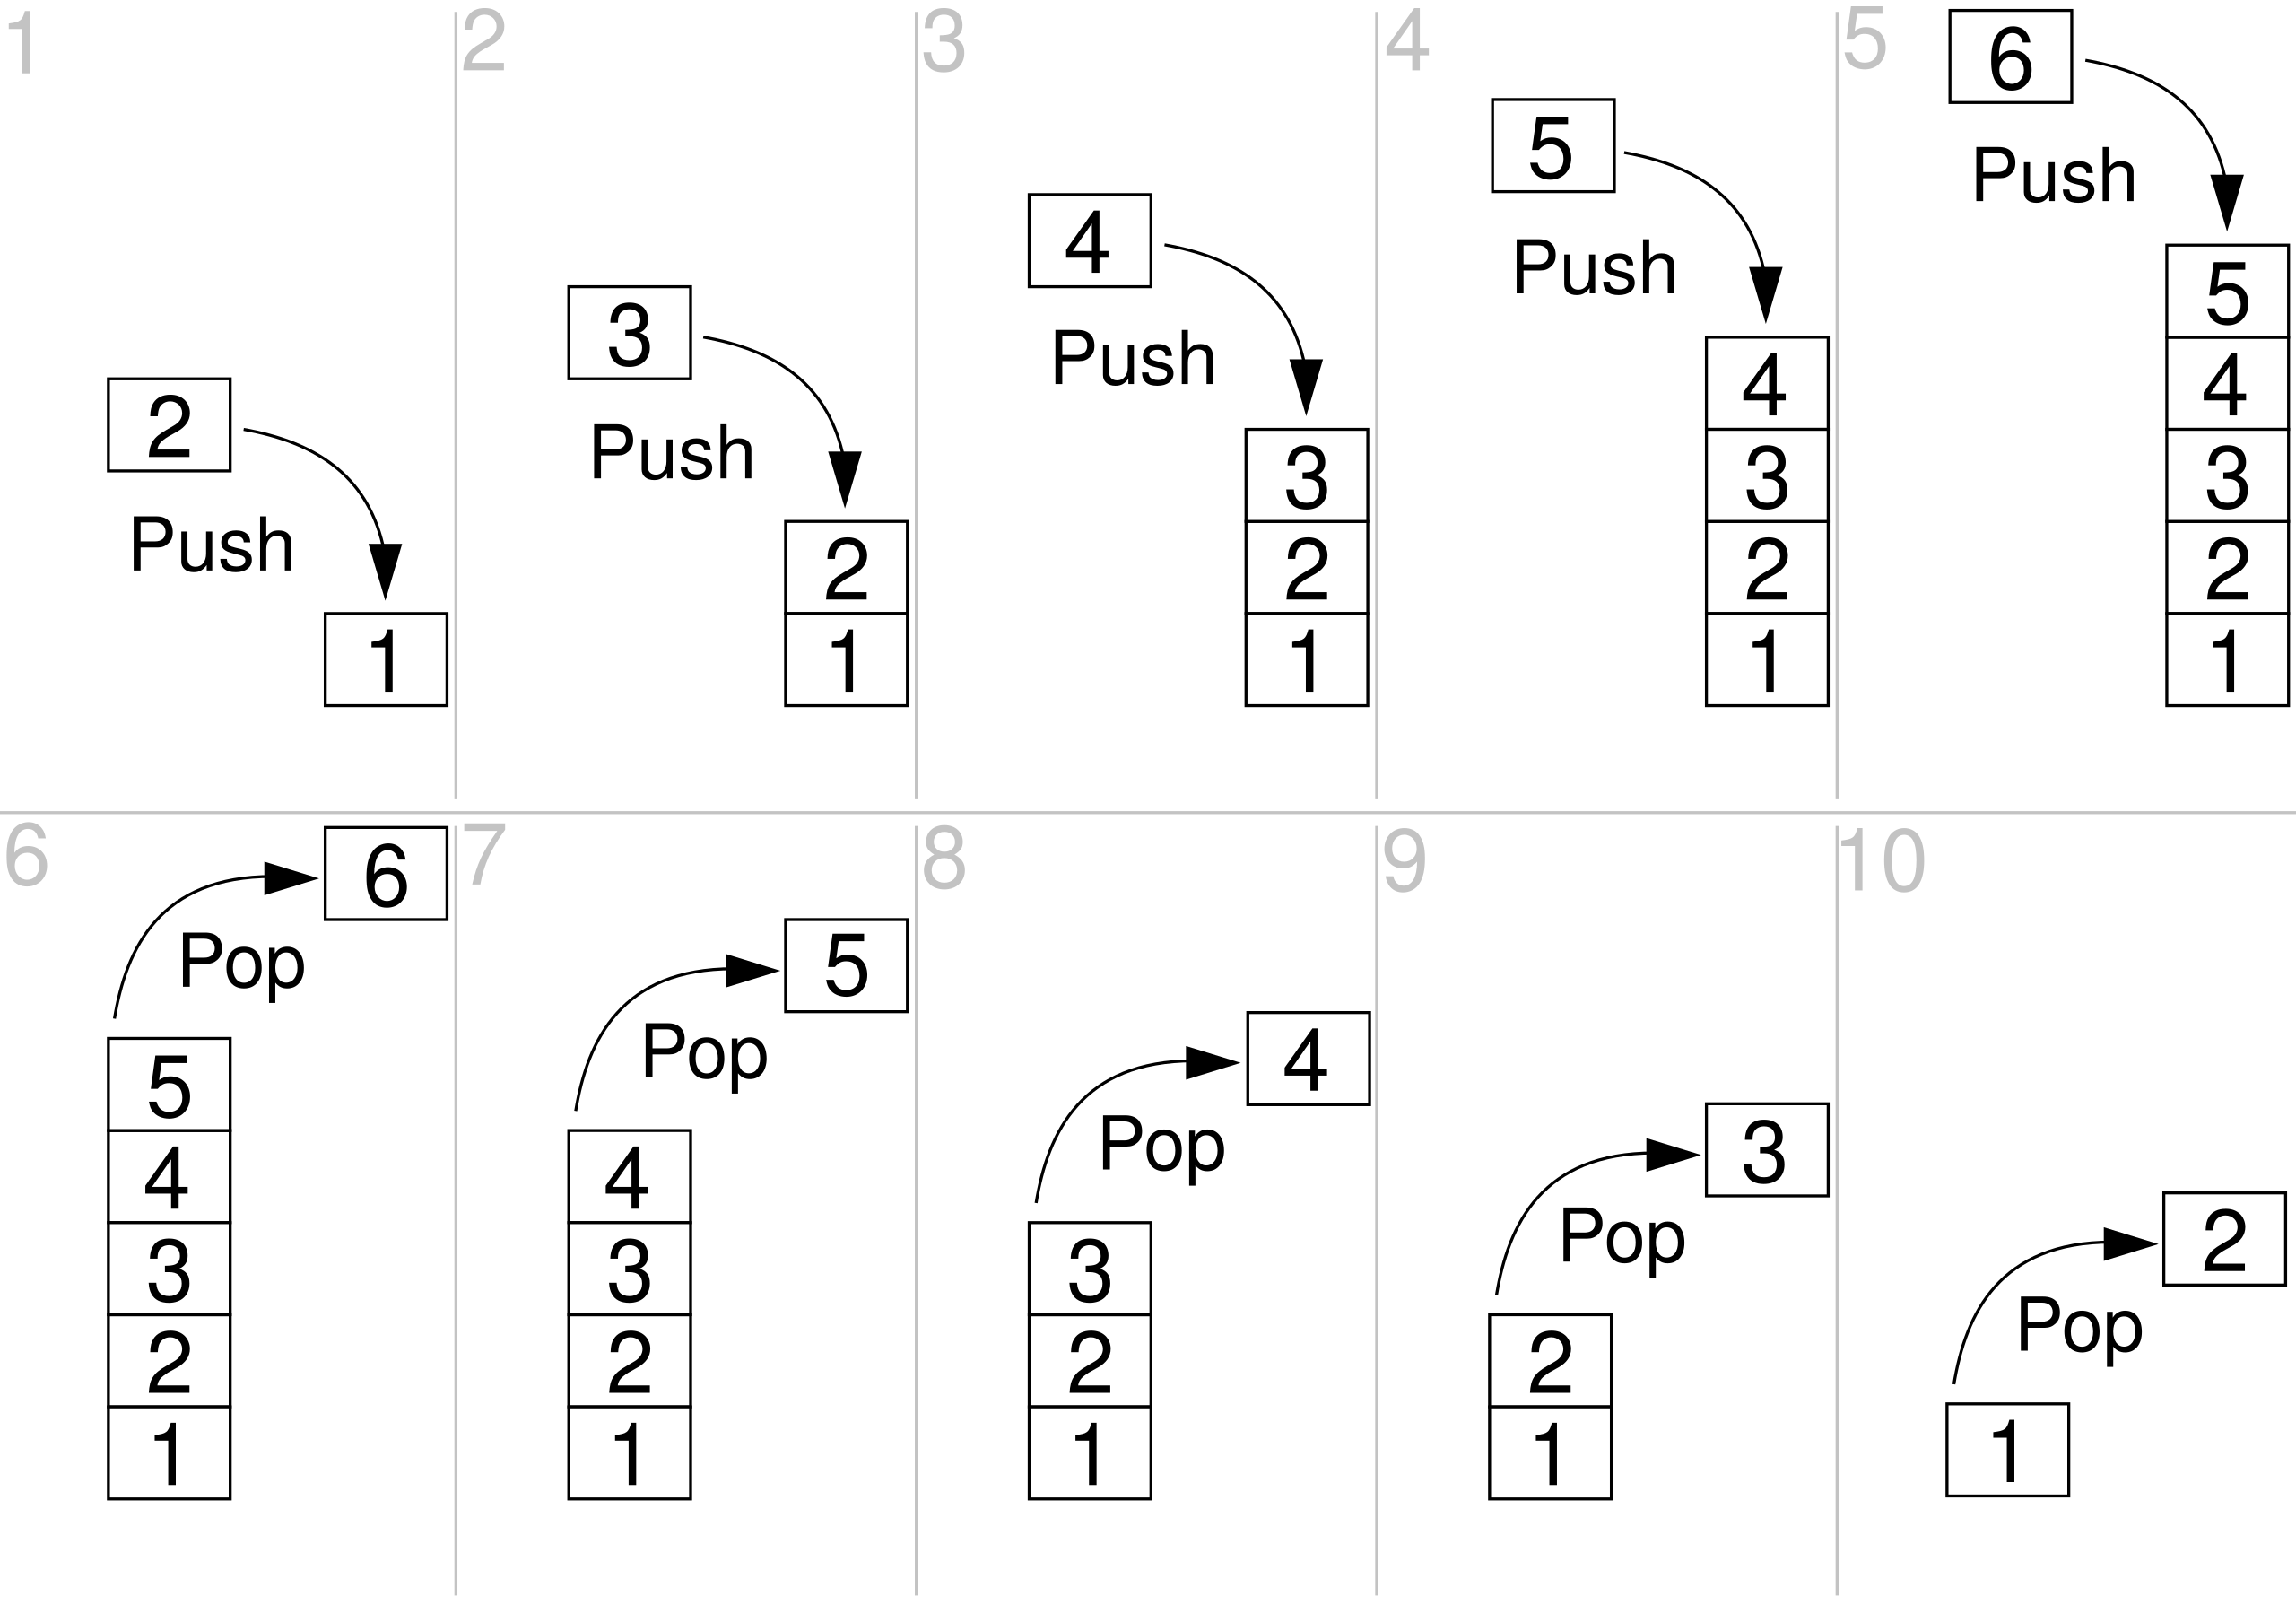
\includegraphics[width=0.9\textwidth]{resources/19-26/stack.png}

В стандартной библиотеке С++ присутствует реализация \cppref[стека]{cpp/container/stack}, объявленная в соответствующем
\cppref[заголовке]{cpp/header/stack}. Стоит отметить, что шаблон \mverb{std::stack<T>} не является
структурой данных сам по себе, а лишь предоставляет интерфейс стека поверх какой-либо другой структуры (по умолчанию, \cppref[\texttt{std::deque<T>}]{cpp/container/deque}).
Помимо этого, в качестве стека можно тривиально использовать динамический массив \cppref[\texttt{std::vector<T>}]{cpp/container/vector} с его
методами \mverb{push_back(T &&)}, \mverb{back()} и \mverb{pop_back()}.
\subsection{Операции над стеком}
Когда речь идет о стеке, подразумевается структура данных со следующими операциями:
\begin{enumerate}
  \item Добавить элемент в верхушку стека (\mverb{push()}).
  \item Удалить элемент из верхушки стека (\mverb{pop()}).
\end{enumerate}

Часто также требуется поддержка операции чтения вершины без ее удаления (\mverb{peek()}, также \mverb{top()}) и
проверки на пустоту (\mverb{empty()}). В эффективной реализации все вышеназванные операции имеют временную сложность
\(O(1)\).

\subsection{Пример реализации стека}
Приведем реализацию стека (С++ 11) на основе статического массива фиксированной длины. Данная реализация будет использовать шаблоны и
\cppref[\texttt{assert(bool)}]{cpp/error/assert} для проверок инвариантов.

\begin{minted}{C++}
template <typename T, size_t N> class Stack {
public:
  Stack() = default;
  ~Stack() = default;

  bool empty() const { return count_ == 0; }
  size_t capacity() const { return N; }
  size_t count() const { return count_; }

  const T &Peek() const {
    assert(count_ > 0 && "Stack is empty.");
    return data_[count_ - 1];
  }
  T &Peek() {
    assert(count_ > 0 && "Stack is empty.");
    return data_[count_ - 1];
  }

  T Pop() {
    assert(count_ > 0 && "Stack is empty.");
    --count_;
    return data_[count_];
  }
  void Push(const T &item) {
    assert(count_ < N && "Stack is full.");
    data_[count_] = item;
    ++count_;
  }
  void Push(T &&item) {
    assert(count_ < N && "Stack is full.");
    data_[count_] = item;
    ++count_;
  }

  T *begin() { return data_; }
  T *end() { return data_ + count_; }
  const T *begin() const { return data_; }
  const T *end() const { return data_ + count_; }

private:
  T data_[N];
  size_t count_{};
};
\end{minted}
\section{Динамические структуры данных: очередь. Основные операции: поиск, вставка, удаление}
Очередь~--- абстрактный тип данных, представляющий собой список данных, организованных по принципу FIFO (англ. first in -- first out, <<первым пришел первым вышел>>).
Очереди могут быть построены на основе других, более фундаментальных структурах данных. Например, очередь может быть внутренне реализована как
список. Об очереди можно судить скорее как об интерфейсе доступа к данным.

Организация по принципу FIFO означает, что элементы могут извлекаться с одного конца (головы), а добавляться~--- с другого (хвоста).

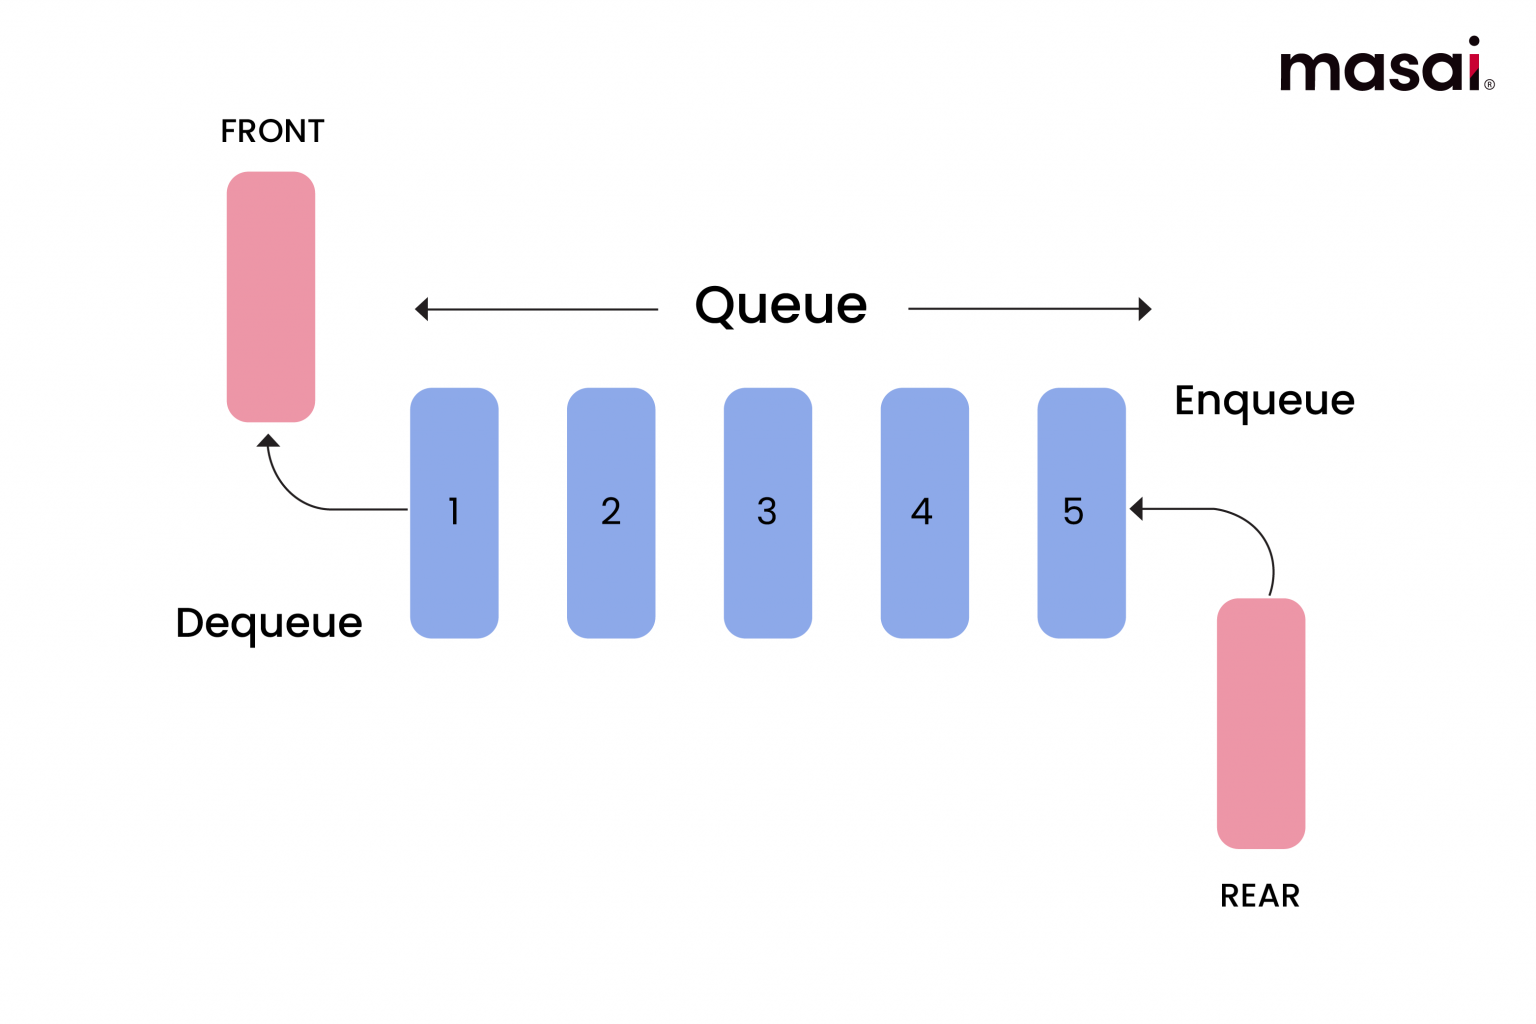
\includegraphics[width=0.9\textwidth]{resources/19-26/queue.png}

В стандартной библиотеке C++ присутствует \cppref[шаблон класса]{cpp/container/queue} \mverb{std::queue<T>}, который является оберткой поверх
какого-либо другого контейнера (по умолчанию, \cppref[\texttt{std::deque<T>}]{cpp/container/deque}).

\subsection{Операции над очередями}
Когда речь идет об очереди, подразумевается структура данных со следующими операциями:
\begin{enumerate}
  \item Добавить элемент в конец (хвост) очереди (\mverb{enqueue()}, в С++ \mverb{push()}).
  \item Удалить элемент из головы очереди (\mverb{dequeue()}, в C++ \mverb{pop()}).
\end{enumerate}
%
Часто также требуется операция чтения головы (\mverb{front()}) и проверки на пустоту (\mverb{empty()}). В эффективной реализации
все указанные операции должны выполнятся за \(O(1)\).

\subsection{Реализация очереди}
Приведем реализацию очереди (С++ 11) на основе кольцевого буфера. Реализация использует шаблоны и \cppref[\texttt{assert(bool)}]{cpp/error/assert}
для проверки инвариантов. Также, в данной реализации запрещена перезапись старых данных~--- в этом случае срабатывает \mverb{assert(bool)} \footnote{Можно заметить, что в операциях с очередью над кольцевым буфером используется операция взятия остатка от деления. Это сравнительно
  медленная операция. Если размер очереди (беззнаковое целое) представляет собой степень \(2\), эту операцию можно заменить на побитовое И. Впрочем, современные
  компиляторы делают это автоматически.}.

\begin{minted}{C++}
template <typename T, size_t N> class Queue {
public:
  Queue() = default;
  ~Queue() = default;

  bool empty() const { return count_ == 0; }
  size_t capacity() const { return N; }
  size_t count() const { return count_; }

  T &Peek() {
    assert(count_ > 0 && "Queue is empty.");
    return data_[start_];
  }
  const T &Peek() const {
    assert(count_ > 0 && "Queue is empty.");
    return data_[start_];
  }

  void Enqueue(T &&item) {
    assert(count_ < N && "Queue is full.");
    data_[end_] = item;
    end_ = (end_ + 1) % N;
    ++count_;
  }
  void Enqueue(const T &item) {
    assert(count_ < N && "Queue is full.");
    data_[end_] = item;
    end_ = (end_ + 1) % N;
    ++count_;
  }

  T Dequeue() {
    assert(count_ > 0 && "Queue is empty.");
    T item = data_[start_];
    start_ = (start_ + 1) % N;
    --count_;
    return item;
  }

private:
  T data_[N];
  size_t start_{};
  size_t end_{};
  size_t count_{};
};
\end{minted}
